\begin{frame}{Comparison Results}
      \centering
      \vfill
      \textbf{\Large Comparison Results}
      \vfill
\end{frame}

\begin{frame}{Performance Evaluation and Transformations}

To evaluate DirichletRF's performance, we compare it with two alternative approaches:
\begin{itemize}
    \item[1)] \textbf{ILR-RF:} A Random Forest model based on log-ratio transformations. 
    The compositional data are first transformed into the ILR
    space. Then, a standard Random Forest is applied to the transformed data, and 
    finally, the predictions are mapped back to the simplex for interpretation.

    \item[2)] \textbf{Dirichlet Regression:} A parametric approach that, 
    works directly on the simplex without requiring any transformation.
\end{itemize}

\end{frame}




\begin{frame}{Evaluation Metrics}
\note{
To compare these models, we used  the Aitchison Distance and the Root Mean Square Error, or RMSE.

The Aitchison Distance is the usual Euclidean distance between them.

On the other hand, RMSE is a widely used and well-known metric. Unlike the Aitchison Distance, it does not take into account the geometric structure of the simplex
}
To compare these models, we used  the Aitchison Distance and the Root Mean Square Error, or RMSE.
\vspace{0.2cm}
\textbf{1. Aitchison Distance:}
\[
AC = \frac{1}{n} \sum_{i=1}^n \sqrt{\sum_{j=1}^k \left(\log\frac{Y_{ij}}{g(\mathbf{Y}_i)} - \log\frac{\hat{Y}_{ij}}{g(\hat{\mathbf{Y}}_i)}\right)^2},
\]
\[
\text{where} \quad g(\mathbf{Y}_i) = \left(\prod_{j=1}^k Y_{ij}\right)^{1/k}
\]
\textit{Measures compositional dissimilarity using log-ratio geometry.}

\vspace{0.3cm}
\textbf{2. Root Mean Square Error (RMSE):}
$
\text{RMSE}_k =  \sqrt{\frac{1}{n} \sum_{i=1}^n (Y_{ij} - \hat{Y}_{ij})^2}
$

\vspace{0.3cm}
\textbf{Interpretation:} Lower values for both metrics indicate better predictive accuracy.
\end{frame}








\begin{frame}{}

    \only<1>{
    \note{We generated two datasets — one simple and one more complex. Here, we used three covariates and a three-dimensional compositional response. The response data was generated from a Dirichlet distribution with a simple, linear relationship to the covariates.}
    \textbf{Simple structure simulations}: We use a simple dataset with $3$ Covariate variables, $X_1,X_1, X_{3}$ and with a $3$-dimensional response, $(Y_1,\,Y_2,\,Y_3)$ such that $Y_1+Y_2+Y_3 = 1$. The response is assumed to follow a Dirichlet distribution with the following parameters:
\[
\alpha_1 = 1 + 2 X_1,\quad \alpha_2 =1 + 0.5 X_2,\quad \alpha_3 = 1 + X_3.
\]
\[
(Y_1,\,Y_2,\,Y_3)\sim Dirichlet(\alpha_1,\alpha_2,\alpha_3)
\]
    }
    \only<2>{
    \note{In this table, you can see the results for the this dataset across different sample sizes.
The first and second columns show the performance of each model based on the both metrics measured on the test set.
The last column shows the difference between the Aitchison Distance on the test and train datasets, which gives us insight into overfitting.

Dirichlet Regression performed better than the other models. This result makes sense, because the data was generated using a Dirichlet distribution with a linear structure.

But, Dirichlet Random Forest does not perform well in this case — in fact, it gives the worst performance in terms of Aitchison Distance and RMSE.

It just performs better than CLR-RF and ILR-RF when it comes to overfitting.

So, we can say that in this example, the main advantage of Dirichlet Random Forest compared to the other RF models is that it is more robust against overfitting.}
    
\begin{table}[htbp]
\centering
\small 
\begin{tabular}{|l|l|c|c|c|c|}
\hline
$N$ & Model & Aitchison Distance  & RMSE & Train-Test \\
\hline

{200} 
    & CLR-RF & 1.299 (0.141) & 0.703 (0.039) & 0.684 \\
    & ILR-RF & 1.303 (0.143) & 0.700 (0.040)& 0.686 \\
    & \textcolor{blue}{Dirichlet Regression} & \textcolor{blue}{\textbf{1.233} (0.139)} & \textcolor{blue}{\textbf{0.745} (0.033)}  & \textcolor{blue}{\textbf{0.030}} \\
    & \texttt{Dirichlet-RF} & 1.451 (0.153) & 0.620 (0.052)  & 0.600 \\
\hline
{500}
    & CLR-RF & 1.282 (0.077) & 0.716 (0.019)  & 0.684 \\
    & ILR-RF & 1.284 (0.077) & 0.716 (0.020)& 0.685 \\
    & \textcolor{blue}{Dirichlet Regression} & \textcolor{blue}{\textbf{1.234} (0.078)} & \textcolor{blue}{\textbf{0.752} (0.016)}  & \textcolor{blue}{\textbf{0.035}} \\
    & \texttt{Dirichlet-RF} & 1.450 (0.077) & 0.627 (0.031) & 0.616 \\
\hline
{2000}
    & CLR-RF & 1.249 (0.032) & 0.726 (0.010) & 0.652 \\
    & ILR-RF & 1.252 (0.032) & 0.725 (0.010)  & 0.654 \\
    & \textcolor{blue}{Dirichlet Regression} & \textcolor{blue}{\textbf{1.209} (0.032)} & \textcolor{blue}{\textbf{0.757} (0.008)}  & \textcolor{blue}{\textbf{0.006}} \\
    & \texttt{Dirichlet-RF} & 1.431 (0.041) & 0.635 (0.016) & 0.596 \\
\hline
\end{tabular}
\caption{ Values represent the means and (standard deviations) of the metrics for test datasets. Train-Test Diff represents the absolute difference between train and test Aitchison Distance, indicating model generalisation capability. }
\label{tab:performance-comparison1}
\end{table}}

    \only<3>{
    	    
    \note{
We compared these models on various datasets—both simulated and real-world. The performance comparison showed competitive results among the random forest-based models. Sometimes the Dirichlet Random Forest performed best, sometimes not—but it consistently delivered satisfactory outcomes.
One situation where it outperformed the others was when the structure of the dataset was complex. For example,
  consider three-dimensional compositional responses and with 10 covariates — only 3 of them are informative, and the other 7 have no relationship with the response. 
As you can see, the responses are generated from a normal distribution, and the relationship with the three informative covariates is nonlinear — we used functions like sin(x), exp(x), quantile, and other nonlinear forms.


    }
    Complex structure synthetic simulations: The dataset consisted of 10 predictor variables \((X_1, \ldots, X_{10})\), with only the first three variables \((X_1, X_2, X_3)\) being truly informative for predicting the compositional response. The three-component compositional response vector $\mathbf{Y} = (Y_1,Y_2,Y_3)$ was constructed through complex non-linear transformations of the informative Covariates. }
    \end{frame}
\begin{frame}
    \only<1>{

\begin{columns}
\begin{column}{0.5\linewidth}

% where \( \mathcal{N}(\mu_i, 0.5^2) \) represents a normally distributed random variable with mean \( \mu_i \) and standard deviation \( 0.5 \), and \( \epsilon \) is a small positive constant ensuring non-negativity.  
% The compositional response variables \( Y_1, Y_2, Y_3 \) are then obtained via the normalisation:
We generate the variables \( Z_1, Z_2, Z_3 \) as follows:  
\[
Z_i = \max(\epsilon, \mathcal{N}(\mu_i, 0.5)), \quad 
\]
\[
Y_i = \frac{Z_i}{Z_1 + Z_2 + Z_3}, \quad  i = 1,2,3.
\]
% This transformation ensures that \( (Y_1, Y_2, Y_3) \) lies within the unit simplex, preserving the compositional structure of the data.
\end{column}
		\begin{column}{0.5\linewidth}

\begin{align*}
\mu_{1j} &= g(2(1 + \sin(x_{1j}))+x_{2j}^3) \\
\mu_{2j} &= g(1 + 2.5\exp(x_{3j})+x_{1j}^2) \\
\mu_{3j} &= g(1 + (1+x_{2j})^2+x_{3j}^4)
\end{align*}

\end{column}

\end{columns}

Where
\[
g(x_{ij}) =
\begin{cases} 
    2, & x_{ij} < \text{Quantile}(x_i, 0.3) \\
    3, & \text{Quantile}(x_i, 0.3) \leq x_{ij} <\text{Quantile}(x_i, 0.6) \\
    4, & \text{Quantile}(x, 0.6) \leq x_{ij} \leq \text{Quantile}(x_i, 0.8) \\
    1, & x_i > \text{Quantile}(x_i, 0.8)
\end{cases}
\]

}
\end{frame}
\begin{frame}
\only<1>{
\note{In this complex scenario, the results are reversed. Our Dirichlet-RF is now the best model, and Dirichlet Regression is the worst.

In terms of overfitting, Dirichlet Regression still performs the best. But this is expected — we don’t usually expect a random forest model to outperform a parametric model with a simple structure when it comes to overfitting.
However, Dirichlet-RF still performs better than the other two random forest models. Overfitting is a common issue in decision tree-based models, but based on our experience, Dirichlet-RF shows better generalization and less overfitting.
}
\begin{table}[htbp]
\centering
\small 
\begin{tabular}{|l|l|c|c|c|c|}
\hline
N & Model & Aitchison Distance & RMSE & Train-Test \\

\hline
{200} 
    & CLR-RF & 0.671 (0.152) & 0.898 (0.018) & 0.366 \\
    & ILR-RF & 0.670 (0.151) & 0.899 (0.018) & 0.364 \\
    & Dirichlet Regression & 0.826 (0.155) & 0.844 (0.026)  & 0.068 \\
    & \textcolor{blue}{{Dirichlet-RF}} & \textcolor{blue}{\textbf{0.659} (0.152)} & \textcolor{blue}{\textbf{0.903} (0.017)}  & 0.221 \\
\hline
{500} 
    & CLR-RF & 0.617 (0.072) & 0.912 (0.011) &   0.334 \\
    & ILR-RF & 0.618 (0.072) & 0.911 (0.012) &  0.334 \\
    & Dirichlet Regression & 0.790 (0.075) & 0.855 (0.012)  & 0.029 \\
    & \textcolor{blue}{{Dirichlet-RF}} & \textcolor{blue}{\textbf{0.606} (0.068)} & \textcolor{blue}{\textbf{0.917} (0.010)}  & 0.201 \\
\hline
{2000} 
    & CLR-RF & 0.557 (0.045) & 0.931 (0.006) & 0.302 \\
    & ILR-RF & 0.557 (0.044) & 0.931 (0.006)& 0.301 \\
    & Dirichlet Regression & 0.785 (0.044) & 0.858 (0.006)  & 0.016\\
    &\textcolor{blue}{ {Dirichlet-RF}} & \textcolor{blue}{\textbf{0.544} (0.044)} & \textcolor{blue}{\textbf{0.936} (0.004) }& 0.178 \\
\hline
\end{tabular}
\caption{ Train-Test Diff represents the absolute difference between train and test Aitchison Distance.}
\label{tab:performance-comparison}
\end{table}
}
\only<2>{
\note{In this complex scenario, the results are reversed. Our Dirichlet-RF is now the best model, and Dirichlet Regression is the worst.

In terms of overfitting, Dirichlet Regression still performs the best. But this is expected — we don’t usually expect a random forest model to outperform a parametric model with a simple structure when it comes to overfitting.
However, Dirichlet-RF still performs better than the other two random forest models. Overfitting is a common issue in decision tree-based models, but based on our experience, Dirichlet-RF shows better generalization and less overfitting.
}
\begin{table}[htbp]
\centering
\small 
\begin{tabular}{|l|l|c|c|c|c|}
\hline
N & Model & Aitchison Distance & RMSE & Train-Test \\

\hline
{200} 
    & CLR-RF & 0.671 (0.152) & 0.898 (0.018) & 0.366 \\
    & ILR-RF & 0.670 (0.151) & 0.899 (0.018) & 0.364 \\
    & Dirichlet Regression & 0.826 (0.155) & 0.844 (0.026)  & \textcolor{blue}{\textbf{0.068}} \\
    & \textcolor{blue}{{Dirichlet-RF}} & 0.659 (0.152) & 0.903 (0.017)  & 0.221 \\
\hline
{500} 
    & CLR-RF & 0.617 (0.072) & 0.912 (0.011) &   0.334 \\
    & ILR-RF & 0.618 (0.072) & 0.911 (0.012) &  0.334 \\
    & Dirichlet Regression & 0.790 (0.075) & 0.855 (0.012)  & \textcolor{blue}{\textbf{0.029}} \\
    & \textcolor{blue}{{Dirichlet-RF}} & 0.606 (0.068) & 0.917 (0.010)  & 0.201 \\
\hline
{2000} 
    & CLR-RF & 0.557 (0.045) & 0.931 (0.006) & 0.302 \\
    & ILR-RF & 0.557 (0.044) & 0.931 (0.006)& 0.301 \\
    & Dirichlet Regression & 0.785 (0.044) & 0.858 (0.006)  & \textcolor{blue}{\textbf{0.016} }\\
    &\textcolor{blue}{ {Dirichlet-RF}} & 0.544 (0.044) & 0.936 (0.004) & 0.178 \\
\hline
\end{tabular}
\caption{ Train-Test Diff represents the absolute difference between train and test Aitchison Distance.}
\label{tab:performance-comparison}
\end{table}
}

\only<3>{
\note{In this complex scenario, the results are reversed. Our Dirichlet-RF is now the best model, and Dirichlet Regression is the worst.

In terms of overfitting, Dirichlet Regression still performs the best. But this is expected — we don’t usually expect a random forest model to outperform a parametric model with a simple structure when it comes to overfitting.
However, Dirichlet-RF still performs better than the other two random forest models. Overfitting is a common issue in decision tree-based models, but based on our experience, Dirichlet-RF shows better generalization and less overfitting.
}
\begin{table}[htbp]
\centering
\small 
\begin{tabular}{|l|l|c|c|c|c|}
\hline
N & Model & Aitchison Distance & RMSE & Train-Test \\

\hline
{200} 
    & CLR-RF & 0.671 (0.152) & 0.898 (0.018) & 0.366 \\
    & ILR-RF & 0.670 (0.151) & 0.899 (0.018) & 0.364 \\
    & Dirichlet Regression & 0.826 (0.155) & 0.844 (0.026)  & 0.068 \\
    & \textcolor{blue}{{Dirichlet-RF}} & 0.659 (0.152) & 0.903 (0.017)  & \textcolor{blue}{ \textbf{0.221}} \\
\hline
{500} 
    & CLR-RF & 0.617 (0.072) & 0.912 (0.011) &   0.334 \\
    & ILR-RF & 0.618 (0.072) & 0.911 (0.012) &  0.334 \\
    & Dirichlet Regression & 0.790 (0.075) & 0.855 (0.012)  & 0.029 \\
    & \textcolor{blue}{{Dirichlet-RF}} & 0.606 (0.068) & 0.917 (0.010)  & \textcolor{blue}{ \textbf{0.201}} \\
\hline
{2000} 
    & CLR-RF & 0.557 (0.045) & 0.931 (0.006) & 0.302 \\
    & ILR-RF & 0.557 (0.044) & 0.931 (0.006)& 0.301 \\
    & Dirichlet Regression & 0.785 (0.044) & 0.858 (0.006)  & 0.016\\
    &\textcolor{blue}{ {Dirichlet-RF}} & 0.544 (0.044) & 0.936 (0.004) & \textcolor{blue}{ \textbf{0.178}} \\
\hline
\end{tabular}
\caption{ Train-Test Diff represents the absolute difference between train and test Aitchison Distance.}
\label{tab:performance-comparison}
\end{table}
}
\end{frame}

\begin{frame}{Learning Curve}
\only<1>{


\begin{figure}
    \centering
    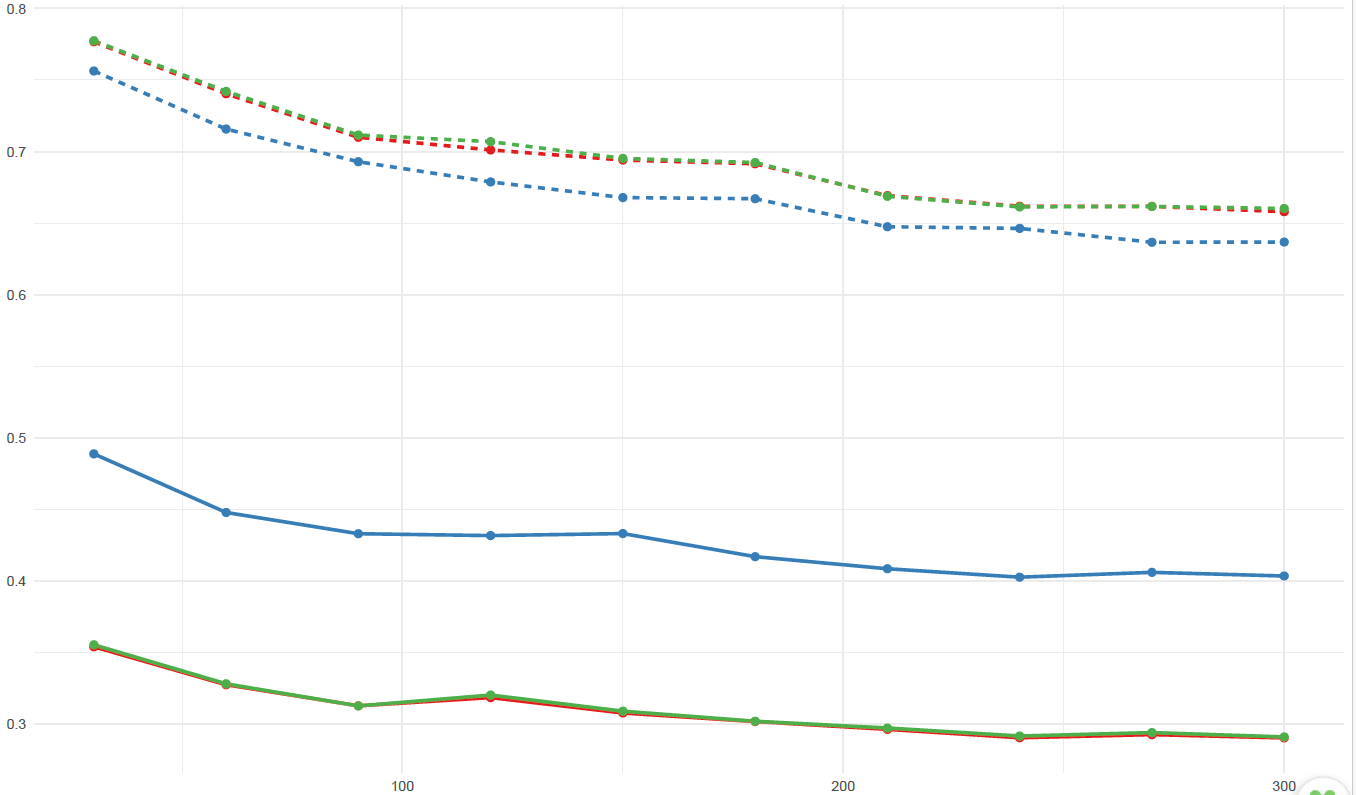
\includegraphics[width=0.75\linewidth]{Learning_curve.png}
    \caption{Aitchison distance as a function of training sample size for all three 
    Random Forest models.}
    \label{fig:enter-label}
\end{figure}
}
\end{frame}



\begin{frame}
\only<1>{
\note{I am not sure to include this slide:

And for further evaluation of \texttt{Dirichlet-RF}, we also looked at its performance in terms of covariate selection.

Here, you can see how often each covariate was selected for splitting across all trees, and how much, on average, it contributed to increasing the log-likelihood.

As I mentioned earlier, only three of the variables were informative — and \texttt{Dirichlet-RF} was able to clearly identify them with high importance.}
\begin{table}[htbp]
\centering
\begin{tabular}{|c|c|c|}
\hline
\textbf{Covariate} & \small{Log-Likelihood Importance} & \small{Frequency-Based Importance} \\
\hline
\textcolor{blue}{$X_1$} & \textcolor{blue}{225.039} & \textcolor{blue}{14} \\
\textcolor{blue}{$X_2$} & \textcolor{blue}{303.618} & \textcolor{blue}{21} \\
\textcolor{blue}{$X_3$} & \textcolor{blue}{272.036} & \textcolor{blue}{19} \\
\textcolor{red}{$X_4$} & \textcolor{red}{16.839}  & \textcolor{red}{2}  \\
\textcolor{red}{$X_5$} & \textcolor{red}{9.972}   & \textcolor{red}{2}  \\
\textcolor{red}{$X_6$} & \textcolor{red}{15.649}  & \textcolor{red}{3}  \\
\textcolor{red}{$X_7$} & \textcolor{red}{0}   & \textcolor{red}{0}  \\
\textcolor{red}{$X_8$} & \textcolor{red}{40.240}  & \textcolor{red}{6}  \\
\textcolor{red}{$X_9$} & \textcolor{red}{5.369}   & \textcolor{red}{1}  \\
\textcolor{red}{$X_{10}$} & \textcolor{red}{23.295}  & \textcolor{red}{3}  \\
\hline
\end{tabular}
\caption{Variable importance scores based on log-likelihood improvement and selection frequency, averaged across all trees in the \texttt{Dirichlet-RF}.}

\label{tab:variable-importance}
\end{table}
\note{
A noteworthy observation is that our model demonstrates effective Covariate selection capabilities through two complementary variable importance measures: log-likelihood importance, which quantifies each variable's contribution to model fit improvement, and frequency-based importance, which measures how often each variable is selected for splitting nodes. Both metrics are averaged across all trees in the random forest. Analysis shows that $X_1$, $X_2$, and $X_3$ receive the highest importance scores across both metrics, identifying them as the informative predictors in our simulation. The remaining variables ($X_4$ through $X_{10}$) receive substantially lower importance scores, confirming the model's ability to distinguish signal from noise.}
}
\end{frame}



\begin{frame}

    \only<1>{
  \note{This real-world dataset is based on a soil texture dataset from KwaZulu-Natal in South Africa. The dataset includes 685 samples, with three compositional parts: sand, silt, and clay. In addition, we used 120 covariates at a spatial resolution of 250 by 250 meters. These covariates include vegetation indices, elevation, precipitation, temperature, and other climate-related variables. The data comes from the Agricultural Research Council – Institute of Soil, Climate and Water.}
\frametitle{Real Data Application: Soil Texture}

\begin{itemize}
    \item \textbf{Data:} 685 samples. \textbf{Compositional parts:} sand, silt, clay. \textbf{120 covariates} at $250\,\text{m} \times 250\,\text{m}$ resolution, including vegetation indices, elevation, precipitation, temperature, and other climate variables.
    
    \item \textbf{Source:} Agricultural Research Council – Institute of Soil, Climate and Water (KwaZulu-Natal, South Africa)
\end{itemize}}
    
    \only<2>{\frametitle{Comparison result}

    \note{\textbf{Dirichlet-RF} outperformed \textbf{CLR-RF} and \textbf{ILR-RF} across all evaluation metrics in this real-data example.

We also compared these models on many simulated datasets. Although we obtained better results in several cases, we cannot claim that this model will always outperform transformation-based Random Forest models in every situation. However, it can be considered a strong and well-structured model for compositional data.}
\begin{table}[ht]
\centering
\begin{tabular}{rrrrr}
  \hline
 & RF-CLR & RF-ILR  & \textcolor{blue}{\texttt{Dirichlet-RF}} \\ 
  \hline
aitchison distance & 1.08 & 1.08  & \textcolor{blue}{\textbf{0.98}} \\ 
  clayRMSE & 20.09 & 20.14  & \textcolor{blue}{\textbf{17.85}} \\ 
  siltRMSE & 13.94 & 13.91  & \textcolor{blue}{\textbf{12.41}} \\ 
  sandRMSE & 29.79 & 29.83  & \textcolor{blue}{\textbf{25.93}} \\ 
  meanRMSE & 22.25 & 22.28  & \textcolor{blue}{\textbf{19.54}} \\ 
   \hline
\end{tabular}
\caption{Results of \texttt{Dirichlet-RF}, \texttt{ILR-RF}, \texttt{CLR-RF}, and an RF without the use of a transformation on the soil texture data in KwaZulu-Natal in South Africa.}
\label{tab:real_results}
\end{table}

    }
\end{frame}





\begin{frame}{Implementation \& Code Access}
\note{This model was developed in Julia, and the full code is available on GitHub at the link provided.

We chose Julia mainly because of its strong computational performance. Implementing the model directly in R or Python would be much slower.

However, if you're working in R or Python, you can still use the model by calling the Julia functions from those languages.
We've included clear instructions in the repository, especially on how to connect Julia with R.

We're also planning to develop an R package with a C++ backend, which we hope to submit to CRAN, so the model will be even easier for R users to access.}
\vspace{1em}

\begin{itemize}[itemsep=1em]
\item[\textcolor{blue}{\large$\blacktriangleright$}] Model developed in \textbf{Julia} for computational efficiency

\item[\textcolor{blue}{\large$\blacktriangleright$}] Code available on \href{https://github.com/Xaleed/DirichletRandomForestJulia.git}{\textcolor{blue}{\textbf{GitHub}}}:

\textcolor{blue}{\small{https://github.com/Xaleed/DirichletRandomForestJulia.git}}
  \begin{center}

    \qrcode{https://github.com/Xaleed/DirichletRandomForestJulia.git}
 \end{center}
\item[\textcolor{blue}{\large$\blacktriangleright$}] Not suitable for direct implementation in \textbf{R} or \textbf{Python}.
However, Julia functions can be called from R or Python.

\end{itemize}

\vspace{1.5em}

\end{frame}

\begin{frame}{}
\only<1>{
\note{One important disadvantage of this approach is the computational cost of estimating the maximum likelihood parameters.

Because there’s no closed-form solution for the maximum likelihood estimator of the Dirichlet distribution parameters we have to solve it numerically.

For example, if we have 10 covariates and 10 candidate split points per covariate, that means we need to numerically solve the MLE problem 600 times at each node.}
\centering
\begin{tikzpicture}[
  node distance=1cm and 1.5cm,
  every node/.style={font=\small},
  data/.style={rectangle, draw, align=center, fill=blue!5, rounded corners, inner sep=5pt},
  split/.style={->, thick}
  ]
  % Parent node
  \node[data] (parent) {
    \textbf{Parent Node} \\[0.15cm]
    Data: $X^{n \times m}$, $Y^{n \times k}$
  };
  
  % Left child
  \node[data, below left=of parent] (left) {
    Data: $X^{n_1 \times m}$, $Y^{n_1 \times k}$ \\[0.15cm]
    $\mathcal{L}(Y^{n_1 \times k}, \alpha_1^L, \alpha_2^L, \alpha_3^L)$
  };
  
  % Right child
  \node[data, below right=of parent] (right) {
    Data: $X^{n_2 \times m}$, $Y^{n_2 \times k}$ \\[0.15cm]
    $\mathcal{L}(Y^{n_2 \times k}, \alpha_1^R, \alpha_2^R, \alpha_3^R)$
  };
  
  % Arrows
  \draw[split] (parent) -- node[midway, left] {$x_{ij} \leq c$} (left);
  \draw[split] (parent) -- node[midway, right] {$x_{ij} > c$} (right);
\end{tikzpicture}

\vspace{0.5cm}



\[
(i^*, c^*) = \operatorname{argmax}_{i,c} \left( \max_{\boldsymbol{\alpha}^L} \mathcal{L}(Y^{n_1 \times k}, \boldsymbol{\alpha}^L) + \max_{\boldsymbol{\alpha}^R} \mathcal{L}(Y^{n_2 \times k}, \boldsymbol{\alpha}^R) \right)
\]
\textbf{Parameter Estimation Complexity:} $6 \times m \times p$ parameters per split:
\[
\text{Total = }6 \times m \times p =  6 \times 10 \times 10 = 600 \text{ optimizations per node}
\]
}
% \only<2>{
% For trees that can potentially grow in all directions to at least 6 levels deep, we have:
% \begin{equation}
% 3 \times m \times p \times \sum_{i=1}^{6} 2^i = 3 \times m \times p \times 126 = 378 \times m \times p
% \end{equation}
% parameters that we estimate dynamically. This number can become very large---for example, when $m=10$ and $p=10$, the total number of parameters is $378 \times 10 \times 10 = 37,800$.
% }
\only<2>{
\note{If we build a tree with just three levels — meaning a tree with 8 leaves — we already need to solve the optimization problem 4,200 times.

This is a large computational cost. And remember, trees can grow much deeper depending on the dataset. As the depth increases, the number of nodes — and therefore the number of parameter estimations — grows exponentially.}
    \centering
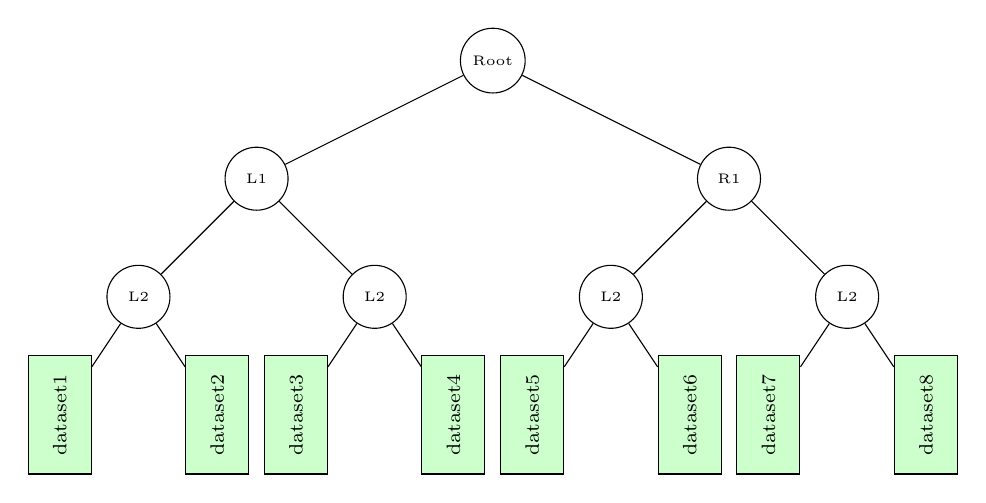
\begin{tikzpicture}[
  level/.style={sibling distance=60mm/#1},
  every node/.style={circle, draw, minimum size=8mm, font=\tiny},
  leaf/.style={rectangle, draw, fill=green!20, minimum width=15mm, minimum height=8mm, font=\scriptsize, rotate=90}
]
\node {Root}
  child {
    node {L1}
    child {
      node {L2}
      child {
        node[leaf] {dataset1}
      }
      child {
        node[leaf] {dataset2}
      }
    }
    child {
      node {L2}
      child {
        node[leaf] {dataset3}
      }
      child {
        node[leaf] {dataset4}
      }
    }
  }
  child {
    node {R1}
    child {
      node {L2}
      child {
        node[leaf] {dataset5}
      }
      child {
        node[leaf] {dataset6}
      }
    }
    child {
      node {L2}
      child {
        node[leaf] {dataset7}
      }
      child {
        node[leaf] {dataset8}
      }
    }
  };
\end{tikzpicture}

With $10$ covariates and $10$ candidates per covariate, the model requires $3 \times 10\times 10 \times (2+2^2+2^3) = 4200$ parameters, all estimated using maximum likelihood estimation. As the tree depth increases, the parameter count grows exponentially.
\note{
This tree diagram illustrates a hierarchical model designed to generate 8 subdatasets, each following a Dirichlet distribution. With 10 covariates and 10 candidates per covariate, the model requires 10×10×(2+2²+2³) = 1,400 parameters, all estimated using maximum likelihood estimation. As the tree depth increases, the parameter count grows exponentially.}
}
% \only<4>{

%  This large parameter space provides the model with sufficient flexibility to accommodate diverse datasets, addressing a key limitation of traditional methods related to the Dirichlet distribution, like Dirichlet regression methods for compositional data analysis. However, this flexibility comes at a significant computational cost, rendering the approach impractical for large-scale datasets. 
% }
% \only<3>{
% The discussion of computational performance remains a significant issue for big datasets in our methodology. We have identified several promising directions for future research and performance improvements. As we discussed, MoM works well as an alternative to MLE, providing good approximations with higher computational speed. We can combine these estimation methods by selectively replacing MLE with MoM in specific nodes where we can predict the results of both methods would be similar, rather than applying MoM to all nodes.
% }
\end{frame}
\begin{frame}{Alternative to MLE}
    \only<1>{
    \begin{block}{}
        One simple way to address this issue is to use the method of moments (MoM) as an alternative to maximum likelihood estimation (MLE). MoM gives an approximate solution but is much faster to compute.
    \end{block}
     \begin{block}{}
        We can also combine both approaches — instead of using MoM in all nodes, we can selectively apply it only in nodes where we expect its results to be close to MLE. This helps reduce computation while still keeping good accuracy.
    \end{block}
            \resizebox{0.65\linewidth}{!}{%

\begin{table}[htbp]
\centering

\begin{tabular}{|l|c|c|c|c|}
\hline
\multirow{Metric} & \multicolumn{2}{c|}{MLE} & \multicolumn{2}{c|}{MoM} \\
\cline{2-5}
 & (Train) & (Test) & (Train) & (Test) \\
\hline
Aitchison Distance & 0.3901 & 0.7391 & 0.4068 & 0.7457 \\
\hline
\end{tabular}
\end{table}}



}
\end{frame}


% \begin{frame}[plain]
% % \begin{center}
% %    
\includegraphics[width=5cm]{logo.png} % Optional logo
% %    \end{center}
%   \begin{center}
%       \vspace{2cm}

%     {\Huge \textbf{Thank You!} \par}
%     % \vspace{1cm}
%     % {\Large Questions or Comments? \par}
%     \vspace{1cm}
   
    
%     \qrcode{https://github.com/Xaleed/DirichletRandomForestJulia.git}
%    % \texttt{khaledmasoumifard@sun.ac.za}
%   \end{center}
% \end{frame}




